\newpage
\section{Concurent processes}
\subsection{Problem:}
\begin{itemize}
    \item Consider three concurrent processes A, B, and C, synchronized by three semaphores mutex, goB, and goC, which are initialized to 1, 0 and 0 respectively: \\
        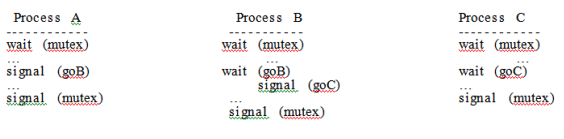
\includegraphics[scale=0.5]{Q_4_a}
        Does there exist an execution scenario in which:
        \begin{itemize}
            \item (i) All three processes block permanently?
            \item (ii) Precisely two processes block permanently?
            \item  (iii) No process blocks permanently?
            Justify your answers.
        \end{itemize}
\end{itemize}

\subsection{Answer:}
